%\begin{figure}[bt]
%\centering
%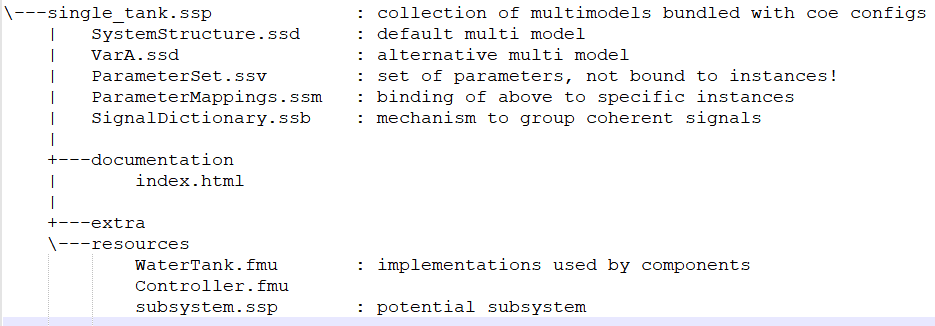
\includegraphics[width=\columnwidth]{Images/ssp_structure.png}
%\caption{}
%\label{fig:ssp_structure}
%\end{figure}



\begin{figure}[bt]
\centering

\begin{Verbatim}[tabsize=4,fontsize=\small,samepage=true,frame=single]
\---single_tank.ssp         : collection of multi models
    | SystemStructure.ssd   : default multi model
    | VarA.ssd              : alternative multi model
    | ParameterSet.ssv      : set of parameters
    | ParameterMappings.ssm : binding params to instances
    | SignalDictionary.ssb  : mechanism to group signals
    |
    +---documentation
    | index.html
    |
    +---extra               : extra files extension mechanism
    |
    \---resources           : implementations of components
      WaterTank.fmu
      Controller.fmu	
      subsystem.ssp         : potential subsystem
\end{Verbatim}

\caption{Example of the file structure of the running example stored as a SSP package. 
The comments on the side describe the role of the file. }
\label{fig:ssp_structure}
\end{figure}